\documentclass[tikz,border=10pt]{standalone}
% No extra TikZ libraries needed.
\begin{document}
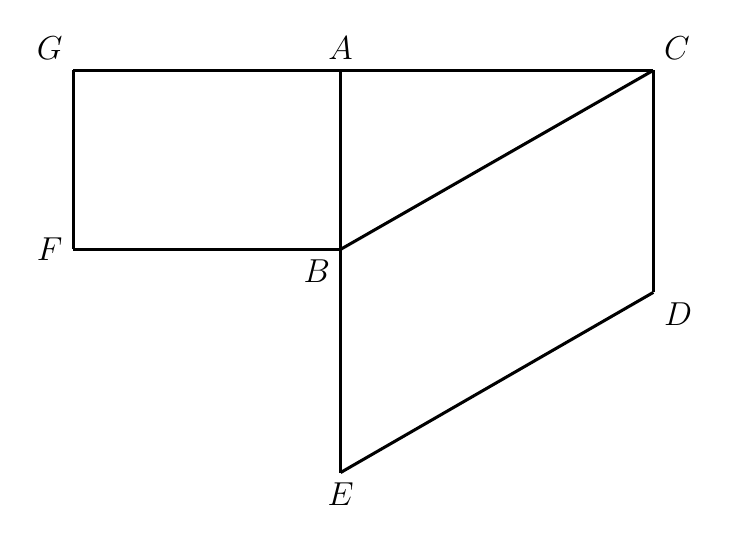
\begin{tikzpicture}[line width=1.1pt, line join=round, font=\fontsize{12}{14.4}\selectfont]
  % Scale s = 0.014388 cm/px, centre (338,256.5) px, y flipped
  \coordinate (G) at (-3.6833,  2.5539);
  \coordinate (A) at (-0.2878,  2.5539);
  \coordinate (C) at ( 3.6833,  2.5539);
  \coordinate (F) at (-3.6833,  0.2806);
  \coordinate (B) at (-0.2878,  0.2806);
  \coordinate (D) at ( 3.6833, -0.2662);
  \coordinate (E) at (-0.2878, -2.5539);

  % Segments
  \draw (G) -- (A) -- (C);   % top edge G-A-C
  \draw (G) -- (F);          % left edge
  \draw (F) -- (B);          % horizontal at y=237
  \draw (A) -- (E);          % vertical x=318, passes through B
  \draw (C) -- (B);          % diagonal C-B
  \draw (C) -- (D);          % right vertical
  \draw (D) -- (E);          % diagonal D-E

  % Labels outside each vertex
  \node[above left]  at (G) {$G$};
  \node[above]       at (A) {$A$};
  \node[above right] at (C) {$C$};
  \node[left]        at (F) {$F$};
  \node[below left]  at (B) {$B$};
  \node[below right] at (D) {$D$};
  \node[below]       at (E) {$E$};
\end{tikzpicture}
\end{document}